\newpage
\setlength{\parskip}{0cm}
\begin{Large}
\section{Архитектура системы}
Опишем архитектуры системы, основанную на требованиях, сформулированных в предыдущей главе
\subsection{Диаграмма классов}
\begin{figure}[h]
    \center{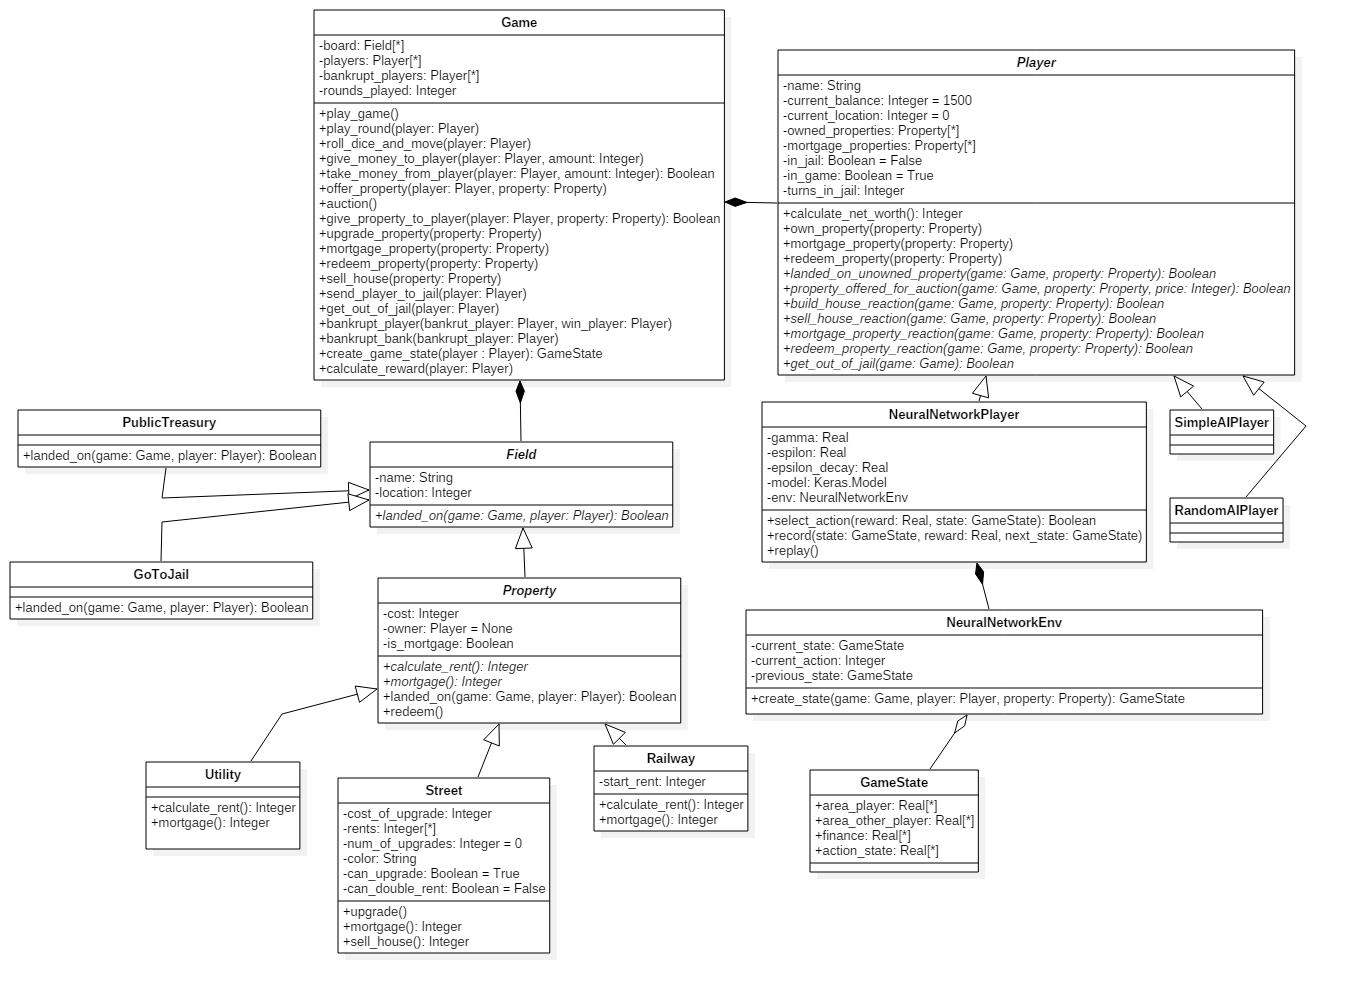
\includegraphics[width=1\linewidth]{class.png}}
    \caption{Диаграмма классов}
\end{figure}
Далее будет описана семантика основных классов программной части и перечислены их функции.
\begin{spacing}{0.9}
\begin{enumerate}
    \item Game - основной класс, в котором реализована логика игры
    \item Field – абстрактный класс поля
    \item Property – абстрактный класс поля, которым может владеть игрок
    \item Chance, Forward, FreeParking, GoToJail, Jail, Tax – поля, которыми нельзя владеть, но которые реализуют различные игровые механики
    \item Utility – класс, реализующий поля «Коммунальное предприятие»
    \item Railway – класс, реализующий поля «Железная дорога»
    \item Street – класс, реализующий поля улиц
    \item Player – абстрактный класс, реализующий интерфейс для разработки ботов, путём реализации логики ответа на события, происходящие в игре
    \item NeuralNetworkPlayer – класс, реализующий нейронную сеть
    \item NeuralNetworkEnv – класс, сохраняющий и формирующий состояния для нейронной сети
    \item RandomAIPlayer – класс, реализующий случайное реагирование на события в игре
    \item SimpleAIPlayer – класс, реализующий простейшую логику бота
    \item GameState – класс, реализующий структуру игрового состояния
\end{enumerate}
\end{spacing}
\subsection{Блок-схема алгоритма аукциона}
Механика аукциона является одной из важнейших в «Монополии», однако полноценная реализация данной механики и удобное использование её средствами нейронной сети является затруднительной и ресурсоёмкой задачей. Для удобного взаимодействия ботов с механикой аукциона был разработан алгоритм, блок-схема которого представлена на рис 4.
\begin{figure}[h!]
    \center{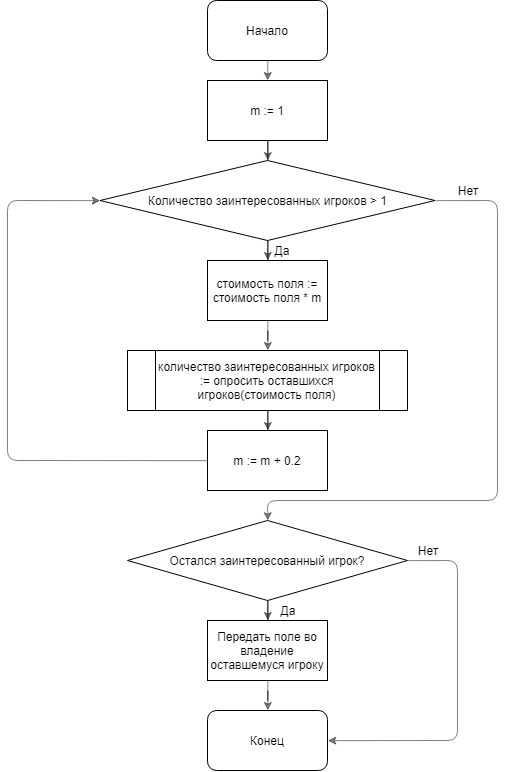
\includegraphics[scale=0.85]{auction.png}}
    \caption{Блок-схема аукциона}
\end{figure}
\newpage
\subsection{Определение характеристик состояния игры и действий игрока}
Для успешного проектирования нейронной сети нужно сформулировать данные, которые будут формировать текущее состояние игры.

Первые 10 значений характеризуют процент владения недвижимостью игровым агентом, представляющим нейронную сеть (8 различных цветов улиц, коммунальные предприятия и железные дороги)

Для улиц значения можно описать таким образом:
\begin{spacing}{0.9}
\begin{enumerate}
    \item 0 – игрок не владеет данным цветом
    \item 0 < xi < 0.6 – игрок владеет хотя бы одним полем данного цвета
    \item 0.6 – игрок монополизировал данное поле
    \item 0.6 < xi < 1 – игрок построил хотя бы один дом на поле данного
    \item 1 – игрок полностью застроил владения данного цвета 
\end{enumerate}
\end{spacing}
Для коммунального предприятия значение описываются так:
\begin{spacing}{0.9}
\begin{enumerate}
    \item 0 – игрок не владеет ни одним полем данного типа
    \item 0.5 – игрок владеет одним полем данного типа
    \item 1 – игрок монополизировал поля данного типа
\end{enumerate}
\end{spacing}
Для железной дороги значения описываются так:
\begin{spacing}{0.9}
\begin{enumerate}
    \item 0 – игрок не владеет ни одним полем данного типа
    \item 0.25 – игрок владеет одним полем
    \item 0.5 – игрок владеет двумя полями 
    \item 0.75 – игрок владеет тремя полями
    \item 1 – игрок монополизировал данный тип поля
\end{enumerate}
\end{spacing}
Следующие 10 значений характеризуют процент владения недвижимостью другими игроками, который рассчитывается по принципу, описанному выше

Следующие 4 значения характеризуют финансовую составляющую агента:
\begin{enumerate}
    \item Отношение активов, принадлежащих агенту к общим активам рассчитываются по формуле 
    \begin{equation}
        x_i = \frac{b_1+n_1}{\sum_{i=1}^{num\_players}b_i + \sum_{i=1}^{num\_players}n_i}
    \end{equation}
    где b – баланс игрока, n – текущая ценность купленной недвижимости
    \item Отношение текущего баланса к начальному, которое рассчитывается по формуле
    \begin{equation}
        x_i = \frac{\frac{b}{1500}}{1+\frac{b}{1500}}
    \end{equation}
    где b -  текущий баланс игрока
    \item Отношение максимальной возможной растраты на аренду/налог к текущему балансу, которое рассчитывается по формуле
    \begin{equation}
        x_i = \frac{\frac{maxrent-b}{b}}{1+|\frac{maxrent-b}{b}|}
    \end{equation}    
    где maxrent – максимально возможная растрата, b – текущий баланс
    \item Отношение купленной недвижимости к общей купленной недвижимости, которое рассчитывается по формуле
    \begin{equation}
        x_i = \frac{p_1}{\sum_{i=1}^{num\_players}p_i}
    \end{equation}
\end{enumerate}

Последнее значение характеризует позицию недвижимости по которому требуется решение, которое формируется в значениях [0, 1]. Например, для поля синего цвета значение будет 0.2.

Для определения размера выходного слоя нейронной сети необходимо определить возможные действия в игре, они будут формировать вектор Action. Предполагается 3 действия:
\begin{spacing}{0.9}
\begin{enumerate}
    \item Купить – купить владение, купить дом во владении, выкупить дом из залога, купить владение на аукционе
    \item Продать – продать дом, заложить владение
    \item Ничего не делать
\end{enumerate}
\end{spacing}
\subsection{Архитектура проектируемой нейронной сети}
Была выбрана следующая архитектура нейронной сети (рис. 4), позволяющая оптимально сочетать в себе скорость обучения и точность решения предоставленных задач.

Нейронная сеть имеет 4 слоя и выглядит следующим образом:
\begin{spacing}{0.9}
\begin{enumerate}
    \item Входной слой определяется размерностью вектора State, описанному в главе ранее.
    \item Первый скрытый слой содержит 200 нейронов. У данного слоя используется функция активации ReLU.
    \item Второй скрытый слой содержит 75 нейронов. У данного слоя используется функция активации ReLU.
    \item Выходной слой определяется размерностью вектора Action. В каждом нейроне на выходе будет значение предполагаемой награды при совершении подобного действия.
\end{enumerate}
\end{spacing}
\newpage
\begin{figure}[h]
    \center{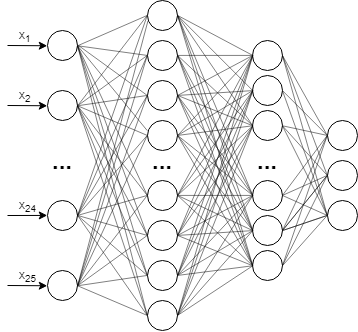
\includegraphics[scale=0.75]{nn.png}}
    \caption{Архитектура нейронной сети}
\end{figure}
\subsection{Функция награды}
Основной задачей игры является завладеть большим количеством полей чем противники и при этом иметь достаточно количество денег для непредвиденных растрат. Для успешного обучения нейронной сети методом Q-learning необходимо сформулировать функцию награды, которая будет выдаваться нейронной сети после каждого выполненного хода. 
\begin{figure}[h!]
    \center{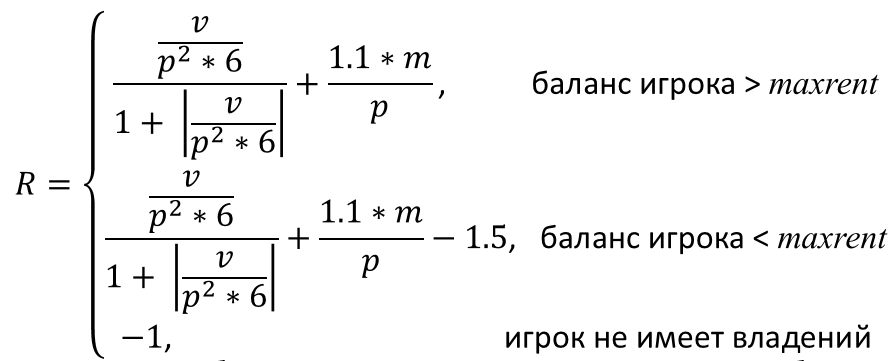
\includegraphics[scale=0.65]{reward.png}}
    \caption{Функция награды}
\end{figure}

где v – разница между приобретенными владениями игрока и приобретенными владениями других игроков, p – количество игроков, m – отношение баланса игрока к балансу всех игроков. Награда игрока будет находиться в значениях [-1;1].
\subsection*{Выводы}
\addcontentsline{toc}{subsection}{Выводы}
В соответствии с требованиями была спроектирована структура разрабатываемой системы, были определены характеристики состояния системы и выделены возможные действия игрока. 

В соответствии с характеристиками состояния и возможных действий игрока была спроектирована нейронная сеть и определена функция награды 
\end{Large}